\chapter{Optimizarea Cererilor SQL}
\label{sec:optimizare_sql}

\section{Cerere}

„Să se compare performanța departamentelor pe ani, afișând numărul total de tichete, venitul estimat și timpul mediu de rezolvare.”

\begin{verbatim}
SELECT d.nume, t.an, COUNT(f.ticket_id), SUM(f.cost_estimativ), 
                     AVG(f.timp_rezolvare_ore)
FROM TickLy_DW.fact_ticket f
JOIN TickLy_DW.dim_departament d ON f.departament_key = d.departament_key
JOIN TickLy_DW.dim_time t ON f.date_creare_key = t.date_key
GROUP BY d.nume, t.an;
\end{verbatim}

\begin{figure}[H]
    \centering
    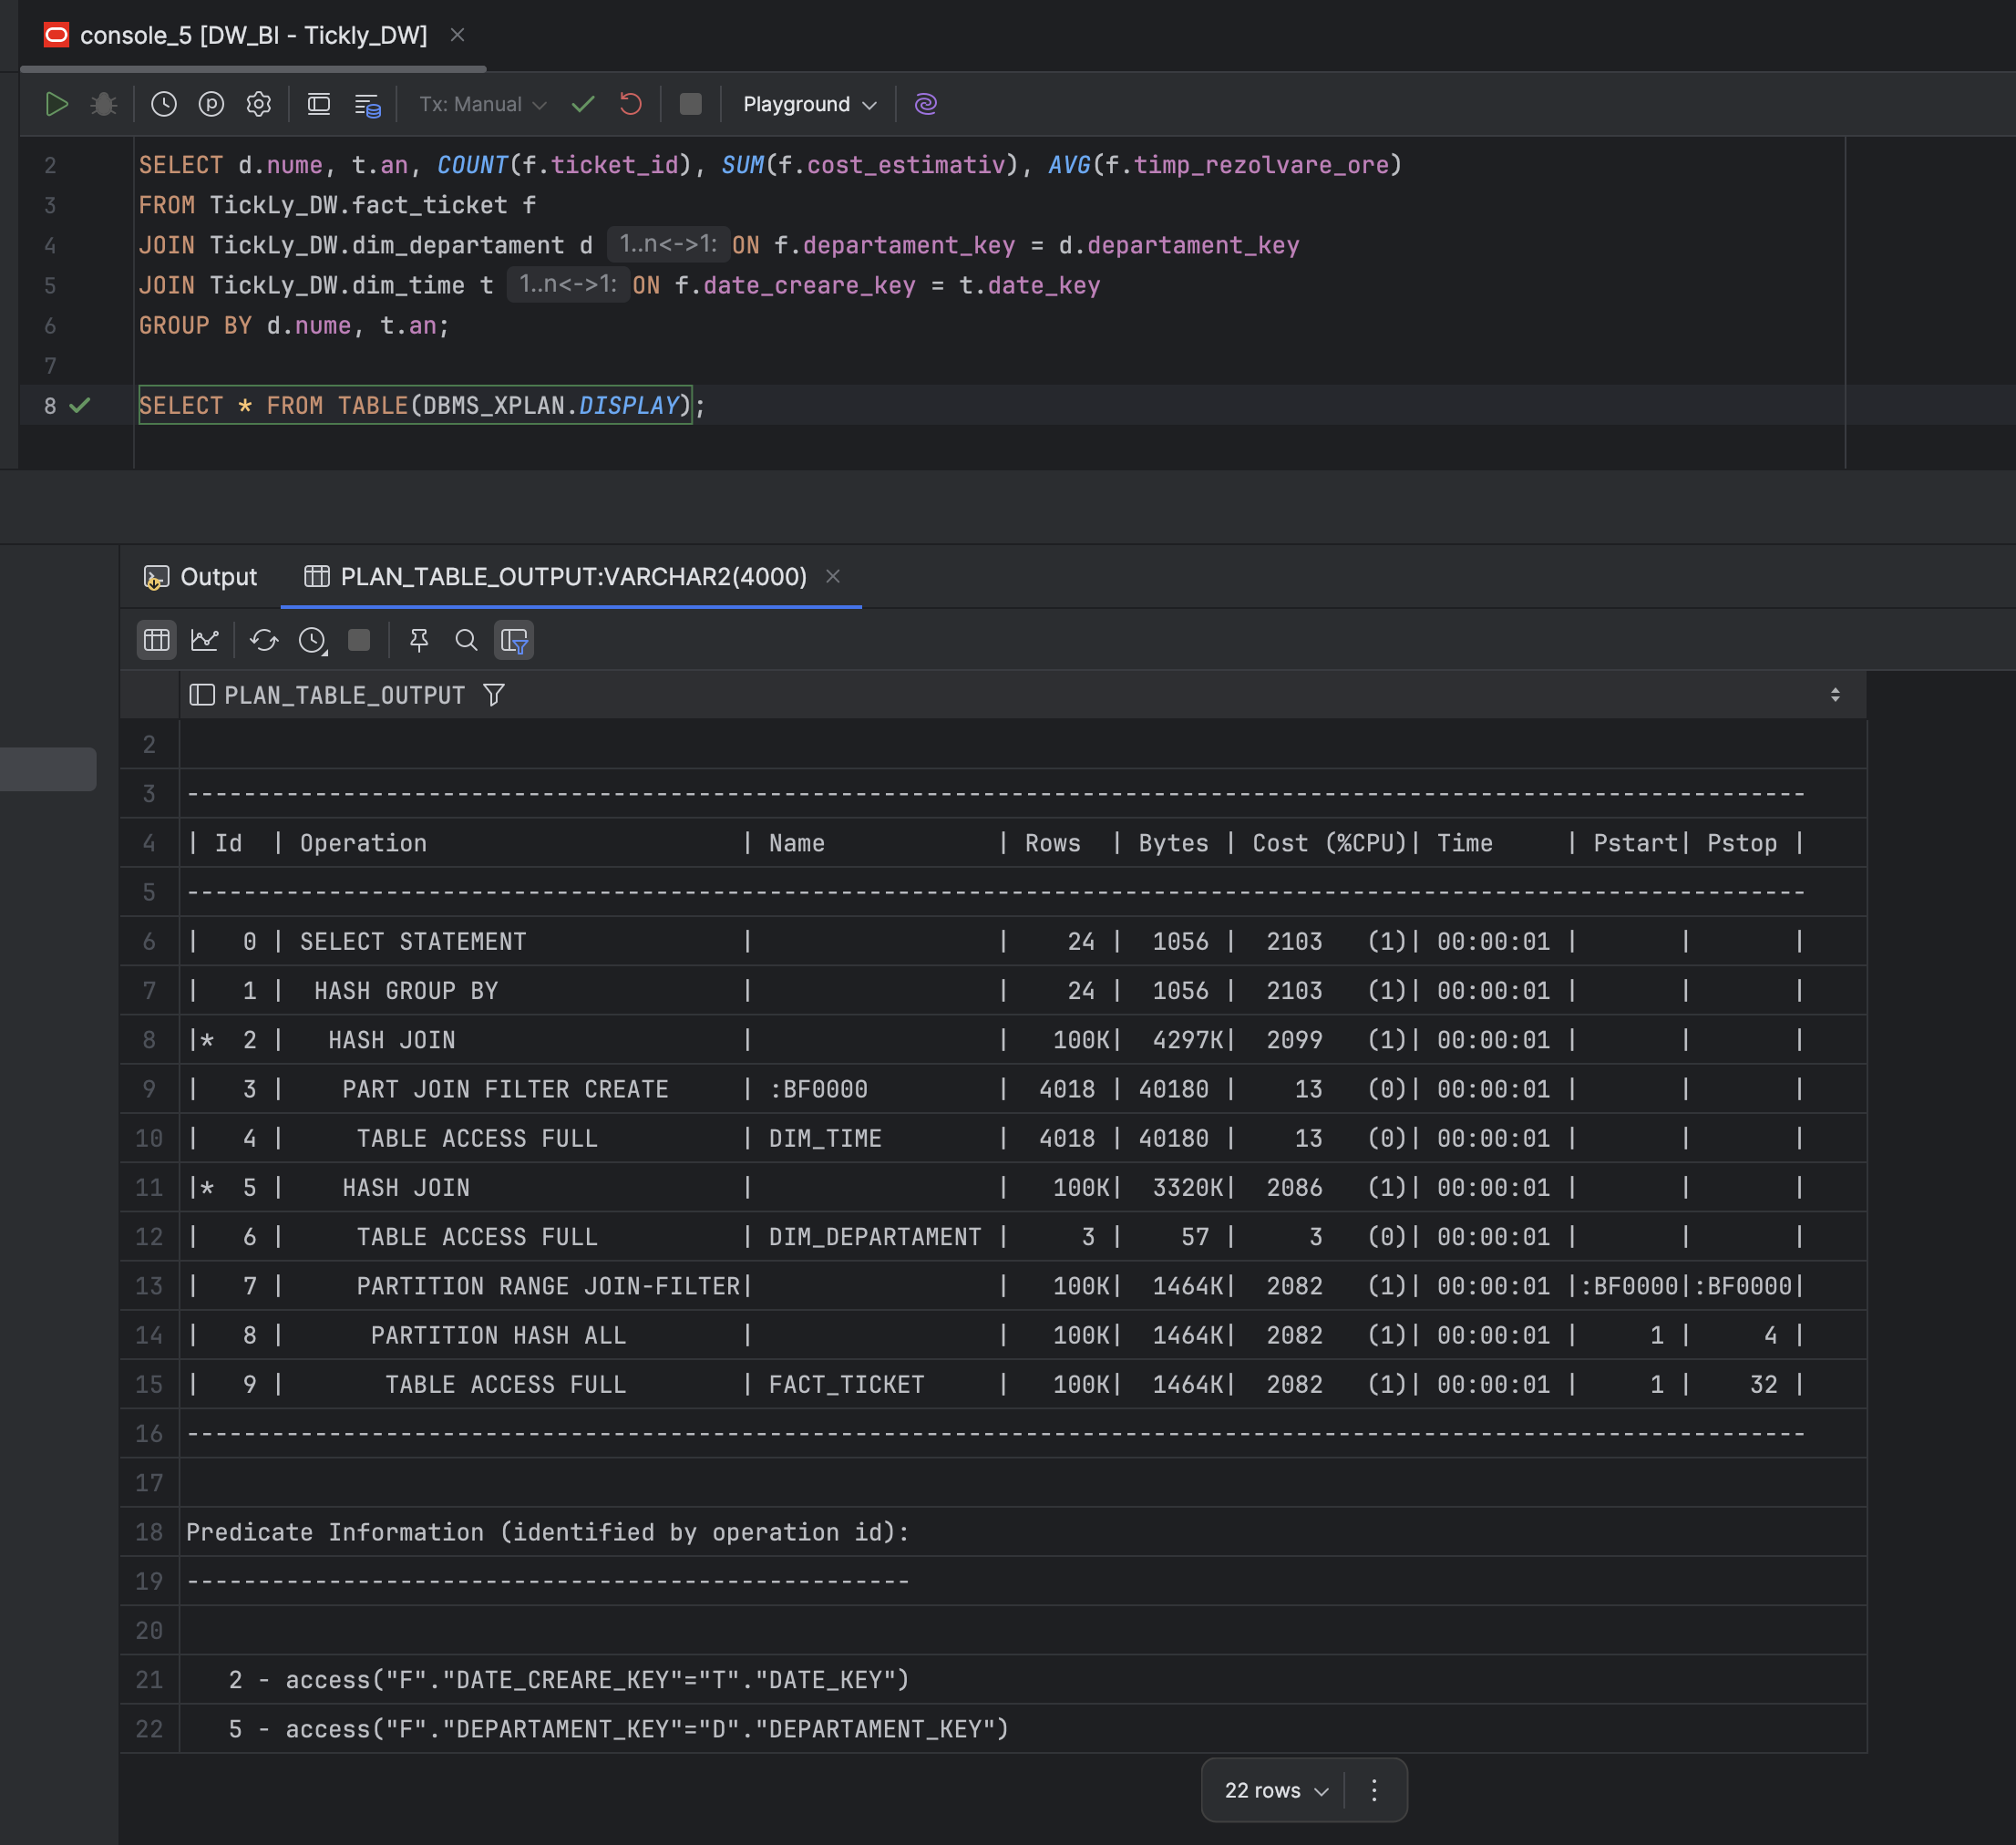
\includegraphics[width=0.6\textwidth]{../../scripts/tests/assets/sql_neoptimizat.png}
    \caption{EXPLAIN SQL Neoptimizat}
    \label{fig:sql_neoptimizat}
\end{figure}

\section{Materialized View}

Pentru optimizare, am creat vederea materializată \texttt{mv\_dept\_yearly\_stats} cu opțiunea \texttt{ENABLE QUERY REWRITE}. Aceasta pre-calculează și stochează rezultatele agregărilor.

\begin{verbatim}
CREATE MATERIALIZED VIEW TickLy_DW.mv_dept_yearly_stats
BUILD IMMEDIATE
REFRESH COMPLETE ON DEMAND
ENABLE QUERY REWRITE AS
SELECT 
    d.nume AS departament_nume,
    t.an,
    COUNT(f.ticket_id) AS mv_total_tichete,
    SUM(f.cost_estimativ) AS mv_venit_total,
    COUNT(f.cost_estimativ) AS mv_count_venit,
    SUM(f.timp_rezolvare_ore) AS mv_sum_timp,
    COUNT(f.timp_rezolvare_ore) AS mv_count_timp
FROM TickLy_DW.fact_ticket f
JOIN TickLy_DW.dim_departament d ON f.departament_key = d.departament_key
JOIN TickLy_DW.dim_time t ON f.date_creare_key = t.date_key
GROUP BY d.nume, t.an;
\end{verbatim}

\begin{figure}[H]
    \centering
    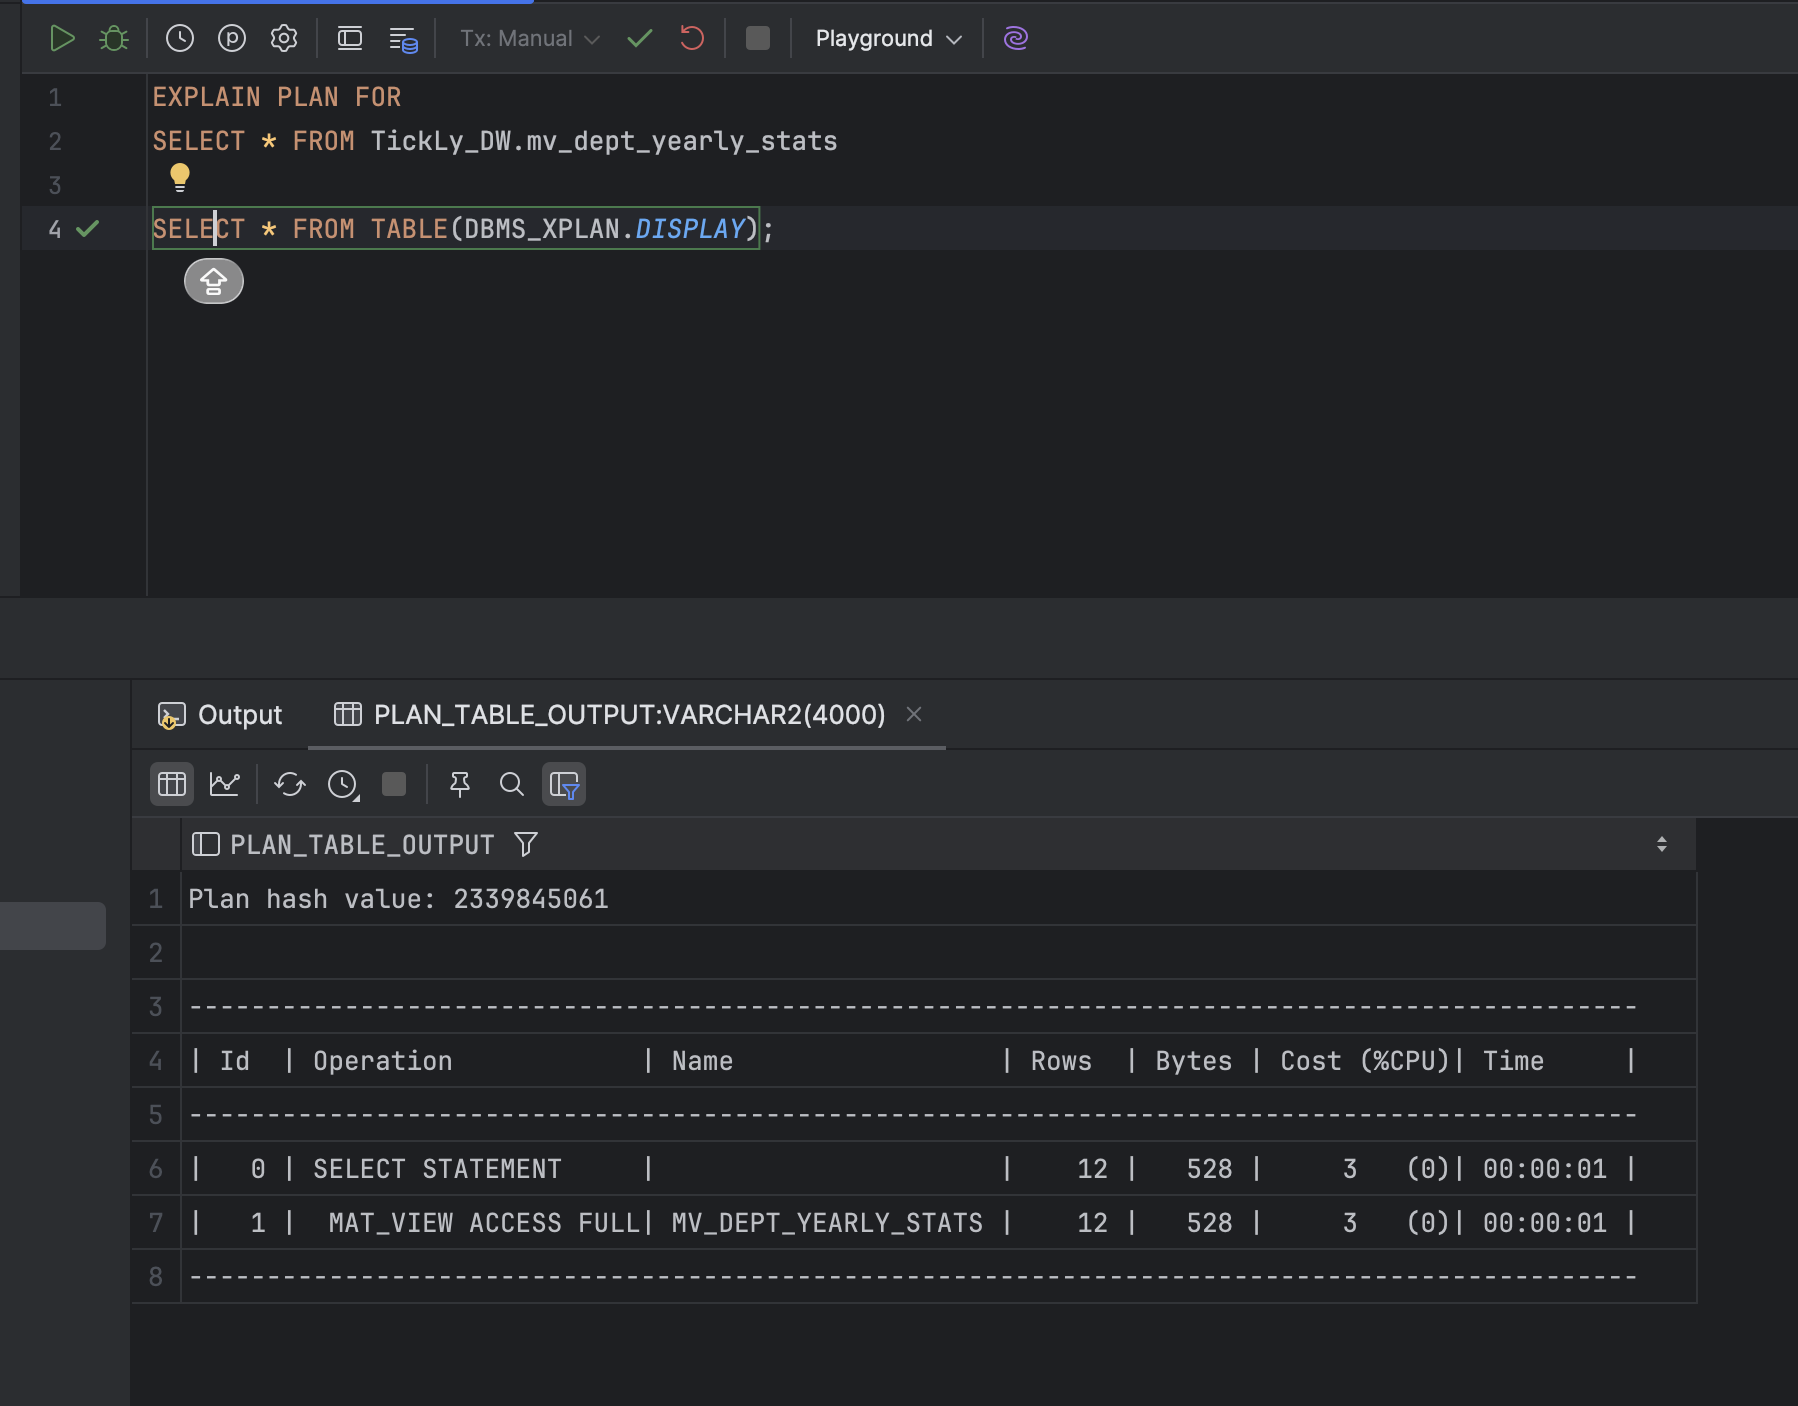
\includegraphics[width=0.6\textwidth]{../../scripts/tests/assets/sql_optimizat.png}
    \caption{EXPLAIN SQL optimizat}
    \label{fig:sql_optimizat}
\end{figure}


\subsection{Avantaje și Dezavantaje}

\begin{itemize}
    \item \textbf{Avantaj (Viteză):} Răspunsul vine instantaneu pentru că citește dintr-un tabel fizic pre-calculat.
    \item \textbf{Dezavantaj (Latență):} Datele nu sunt actualizate în timp real.
    \item \textbf{Dezavantaj (Spațiu):} Ocupă spațiu suplimentar pe disc.
\end{itemize}
